\section{More about State Relation Between Low- and High-level Program}
\label{sec:more-staterel}

After introducing the definitions of low- and high-level program, 
we establish the state relation between low- and high-level program 
in this section. Establishing their state relation is not a trivial 
task, because there are two major differences low- and high-level 
program states. \textbf{First}, all the procedures' contexts of 
a specific thread are saved in high-level frame list $\hWstk$. 
However, for low-level program, part of the contexts are saved in 
register windows (modeled as low-level frame list $\Wstack$), the 
other part of the contexts are saved in corresponding stack frame 
in memory, because the number of register windows is limited; 
\textbf{Second}, the high-level concurrent Pseudo-SPARCv8 program 
is multithreaded, but the low-level SPARCv8 program does not have 
the concept of thread pool. 

\begin{figure}[!t]
    \centering
    \small
    \[
        \begin{array}{c}
            \infer
            {
                \stkRel{(\block, \nil, \emptyset)}{\nil}
            }
            {} \qquad \quad
            \infer
            {
                \stkRel{(\block, \nil, \Mem_K)}{(\block, \fm_1, \fm_2) \stCons \hWstk}
            }
            {
                \Mem_K = \framMem{(\block, \fm_1, \fm_2)} \uplus \Mem_K' 
                \quad \ \ \fm_2[6] = (\block', 0) \quad \ \  
                \stkRel{(\block', \nil, \Mem_K')}{\hWstk}
            } \\
            \\
            \infer
            {
                \stkRel{(\block,
                	\fm_1 \stCons \fm_2 \stCons \Wstack, \Mem_K)}
                    {(\block, \fm_1', \fm_2') \stCons \hWstk}
            }
            {
                \fm_1 = \fm_1' \quad \ \ \fm_2 = \fm_2' \quad \ \  
                \Mem_K = \framMem{(\block, \notCare, \notCare)} \uplus \Mem_K'
                \quad \ \ 
                \fm_2[6] = (\block', 0) \quad \ \ 
                \stkRel{(\block', \Wstack, \Mem_K')}{\hWstk}
            }
        \end{array}
    \]
    \caption{Relation for low- and high-level FrameList}
    \label{fig:relation-low-high-level-framelist}
\end{figure}

\paragraph{\bf Relation for low- and high-level FrameList.} 
The relation between low- and high-level frame list is defined in 
\Fig{\ref{fig:relation-low-high-level-framelist}}. We represent 
this relation as form 
``$\stkRel{(\block, \Wstack, \Mem_K)}{\hWstk}$", 
The tuple of $\block$, 
$\Wstack$ and $\Mem_K$ is the state of stack in low-level program, 
because, in the low-level program, part of the produces' contexts are 
saved in frame list $\Wstack$, which can also be understand as a 
prefix the whole frame list describe in assertion $\stackAstP{\notCare}{\Wstack}$, 
the other part of the contexts are saved in corresponding frame list 
represent as $\Mem_K$. The high-level frame list $\hWstk$ represents the 
state of stack in high-level program. 
\Fig{\ref{fig:Abstraction of Register Windows and Memory}} gives a 
more intuition understanding of this relation. Here, some part of 
the contexts $\Wstack$ (the pink part in the left side of the 
\Fig{\ref{fig:Abstraction of Register Windows and Memory}}) 
are saved in register windows, and the other part of contexts 
$\Mem_K$ (the green part in the left side of the 
\Fig{\ref{fig:Abstraction of Register Windows and Memory}}) are 
saved in stack frame in memory. However, in high-level state, 
they are abstracted as list named high-level frame list $\hWstk$. 
% \begin{figure}[!t]
    \centering
    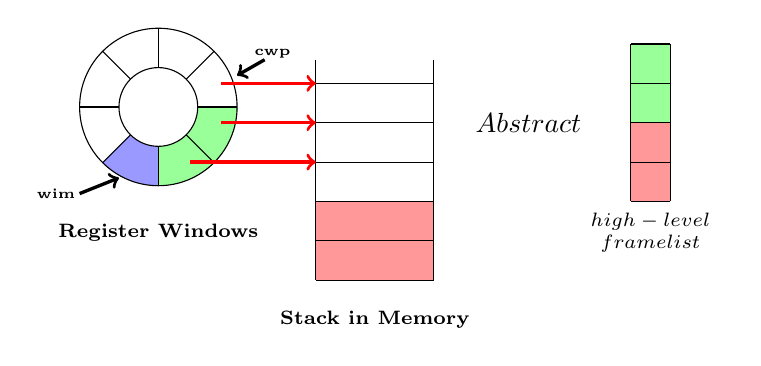
\begin{tikzpicture}
        \fill[green!40!white] (0,0) -- (0,-1cm) arc (-90:0:1cm) -- (0,0);
        \fill[blue!40!white] (0,0) -- (0,-1cm) arc (-90:-135:1cm) -- (0,0);
        % \fill[yellow!80!white] (0,0) -- (0,-1cm) arc (-90:-135:1cm) -- (0,0);
        % \fill[blue!40!white] (0,0) -- (-1,0cm) arc (-180:-135:1cm) -- (0,0);
        \draw (0, 0) -- (90:1cm);
        \draw (0, 0) -- (45:1cm);
        \draw (0, 0) -- (0:1cm);
        \draw (0, 0) -- (-45:1cm);
        \draw (0, 0) -- (-90:1cm);
        \draw (0, 0) -- (-135:1cm);
        \draw (0, 0) -- (-180:1cm);
        \draw (0, 0) -- (135:1cm);
        \fill[white] (0, 0) circle (0.5cm);
        \draw (0, 0) circle (1cm);
        \draw (0, 0) circle (0.5cm);
        % \draw[very thick, blue] (0, -0.3) -- (0, -1.2);
        % \draw[very thick, blue] (0, -0.32) -- (0.1, -0.32);
        % \draw[very thick, blue] (0, -1.18) -- (0.1, -1.18);
        \node(wim) at (-1.3, -1.1) {\tiny \bf wim};
        \draw[->, very thick] (-1, -1.1) -- (-0.5, -0.9);

        % \node(wim) at (-1.7, -0.7) {\tiny \bf wim};
        % \draw[->, very thick] (-1.5, -0.6) -- (-1, -0.4);
        

        \node(cwp) at (1.45, 0.67) {\tiny \bf cwp};
        \draw[->, very thick] (1.35, 0.6) -- (1, 0.4);

        \node(regwin) at (0, -1.6) {\scriptsize \bf Register Windows};

        %%%%%%%%%%%%%%%%%%%%%%%%%%%%%%%%%%%%%%%%%%%%%%%%%%%%%%

        \fill[red!40!white] (2, -1.2) rectangle (3.5, -1.7);
        \fill[red!40!white] (2, -1.7) rectangle (3.5, -2.2);

        \draw[-] (2, 0.6) -- (2, -2.2);
        \draw[-] (3.5, 0.6) -- (3.5, -2.2);
        
        \draw[-] (2, 0.3) -- (3.5, 0.3);
        \draw[-] (2, -0.2) -- (3.5, -0.2);
        \draw[-] (2, -0.7) -- (3.5, -0.7);
        \draw[-] (2, -1.2) -- (3.5, -1.2);
        \draw[-] (2, -1.7) -- (3.5, -1.7);
        \draw[-] (2, -2.2) -- (3.5, -2.2);

        \node(stkfm) at (2.75, -2.7) {\scriptsize \bf Stack in Memory};

        %%%%%%%%%%%%%%%%%%%%%%%%%%%%%%%%%%%%%%%%%%%%%%%%%%%%%%%

        \draw[->, very thick, red] (0.8, 0.3) -- (2, 0.3);
        \draw[->, very thick, red] (0.8, -0.2) -- (2, -0.2);
        \draw[->, very thick, red] (0.4, -0.7) -- (2, -0.7);

        %%%%%%%%%%%%%%%%%%%%%%%%%%%%%%%%%%%%%%%%%%%%%%%%%%%%%%

        \node(abstract) at (4.7, -0.2) {$\xLongrightarrow{\text{Abstract}}$};

        %%%%%%%%%%%%%%%%%%%%%%%%%%%%%%%%%%%%%%%%%%%%%%%%%%%%%%

        \fill[green!40!white] (6, 0.8) rectangle (6.5, 0.3);
        \fill[green!40!white] (6, 0.3) rectangle (6.5, -0.2);
        \fill[red!40!white] (6, -0.2) rectangle (6.5, -0.7);
        \fill[red!40!white] (6, -0.7) rectangle (6.5, -1.2);

        \draw[-] (6, 0.8) -- (6, -1.2);
        \draw[-] (6.5, 0.8) -- (6.5, -1.2);

        \draw[-] (6, 0.8) -- (6.5, 0.8);
        \draw[-] (6, 0.3) -- (6.5, 0.3);
        \draw[-] (6, -0.2) -- (6.5, -0.2);
        \draw[-] (6, -0.7) -- (6.5, -0.7);
        \draw[-] (6, -1.2) -- (6.5, -1.2);

        \node(hfrmlist) at (6.25, -1.6) 
            {
                \scriptsize \bf
                $
                \begin{array}{c}
                    \text{high-level} \\
                    \text{framelist}
                \end{array}
                $
            };
    \end{tikzpicture} 
    \caption{Abstraction of Register Windows and Memory}
    \label{fig:Abstraction of Register Windows and Memory}
    \vspace{-0.5em}
\end{figure}

As shown in \Fig{\ref{fig:relation-low-high-level-framelist}}, if 
the low-level frame list $\Wstack$ is $\nil$ and the memory is $\emptyset$, 
and the high-level frame list $\hWstk$ is $\nil$, it means there is no 
context stored. If the frame list is $\nil$ but the high-level frame list 
is $(\block, \fm_1, \fm_2) \stCons \hWstk$, it means that the contexts 
$\fm_1$ and $\fm_2$ are saved in stack frame in memory, whose block identifier 
is $\block$. Here, we use ``$\framMem{(\block, \fm_1, \fm_2)}$" defined below to 
represent the part of memory saving $\fm_1$ and $\fm_2$. This memory contains 
only one block $\block$.  
\[
    \begin{array}{lll}
        \framMem{(\block, \fm_1, \fm_2)} & \define & 
        \{ (\block, 0) \rightsquigarrow \val_0, 
            (\block, 4) \rightsquigarrow \val_1, \dots, 
            (\block, 28) \rightsquigarrow \val_7 \} \\
        & & \quad \ \ \uplus
        \{
            (\block, 32) \rightsquigarrow \val_0', 
            (\block, 36) \rightsquigarrow \val_1', \dots,
            (\block, 60) \rightsquigarrow \val_7'   
        \} \\
        \\[-8pt]
        & 
        \multicolumn{2}{l}
        {
            \text{where} \  
            \fm_1 = \Array{\val_0, \dots, \val_7}, \,  
            \fm_2 = \Array{\val_0', \dots, \val_7'}. 
        }
    \end{array}
\]
If the frame list is $\fm_1 \stCons \fm_2 \stCons \Wstack$ 
and the high-level frame list is $(\block', \fm_1', \fm_2') \stCons \hWstk$, 
it means that the contexts $\fm_1$ and $\fm_2$ have not 
been saved in block $\block'$. So, we require the contexts 
$\fm_1$ and $\fm_2$ saved in low-level frame list and 
the $\fm_1'$ and $\fm_2'$ saved in high-level frame list 
are equal. The block $\block'$ used to save $\fm_1$ and $\fm_2$ 
has not been used yet, so we don't care about its contents. 

\paragraph{\bf Relation for ThreadPool and low-level Memory.} 
In high-level program, the thread local state of each thread 
is saved in a thread pool $\thrdpool$. However, in low-level 
program, the local state of each thread is saved in memory 
(TCB and stack). For example, in \Sec{\ref{sec:ctxswitch}}, 
we introduce that the execution of the context switch module
will save the register state of current thread into its 
TCB and stack in memory. So, the thread pool in high-level 
program can be viewed as an abstraction of low-level memory 
used to store the contexts of threads. 

\begin{figure}[!t]
    \centering
    \[
        \begin{array}{lcl}
            \ctxfm(\RFile, \Wstack) & \define & 
            \left\{
            \begin{array}{ll}
                \Wstack_1 & \quad \cif \
                \RFile(\regcwp) = \cwp, \, 
                \RFile(\regwim) = 2^{n}, \, 
                \regcwp \neq n, \\
                & \qquad
                \Wstack = \Wstack_1 \lstApp \Wstack_2, \, 
                0 \leq \cwp, n \leq N, \, 
                | \Wstack_1 | = 2 \times 
                    {(N + n - \cwp - 1)}\modOP{N} \\
                \\[-8pt]
                \perp & \quad \otherwise
            \end{array} 
            \right. \\
            \\
            \Rinj{\RFile}{\hRfile} & \define & 
            (\forall \, i \in \{ 0, \dots, 31 \}. \, 
                \RFile(\reg{i}) = \hRfile(\reg{i}))
                \, \land \, 
                (\forall \, \sr. \, \exists \, \word. \  
                \RFile(\sr) = \word) \\
            & & \quad \, \land \, 
            \RFile(\regn) = \hRfile(\regn) \, \land \, 
            \RFile(\regz) = \hRfile(\regz) \, \land \, 
            \RFile(\regc) = \hRfile(\regc) \, \land \, 
            \RFile(\regv) = \hRfile(\regv) \\
        \end{array}
    \]
    \[
        \begin{array}{c}
            \\[-5pt]
            \infer
            {
                \curStRel{(\Mem_c, (\RFile, \Wstack))}
                    {(\thrdid, ((\hRfile, \block, \hWstk), \pc, \npc))}
            }
            {
                \begin{array}{c}
                    \Mem_c = \Mem_{\text{ctx}} \uplus \Mem_K 
                    \quad \ \ 
                    \dom(\Mem_{\text{ctx}}) = \DomCtx{(\thrdid, \block)}
                    \quad \ \ 
                    \RFile(\spreg) = (\block, 0) 
                    \\
                    \ctxfm(\RFile, \Wstack) = \Wstack' \quad \ \ 
                    \RFile(\fpreg) = (\block', 0) \quad \ \ 
                    \stkRel{(\block', \Wstack', \Mem_K)}{\hWstk} 
                    \quad \ \ 
                    \Rinj{\RFile}{\hRfile} 
%                    \quad \ \ 
%                    \hRfile(\spreg) = (\block, 0)
                \end{array}
            } \\
            \\
            \infer
            {
                \rdyStRel{\Mem_1 \uplus \Mem_2}{\thrdpool_1 \uplus \thrdpool_2}
            }
            {
                \rdyStRel{\Mem_1}{\thrdpool_1} \quad \ \ 
                \rdyStRel{\Mem_2}{\thrdpool_2}
            } \qquad \quad
            \infer
            {
                \rdyStRel{\Mem}{\{ \thrdid \rightsquigarrow \hthrdlocalst \}}
            }
            {
                \restoreCtx{\Mem}{\thrdid}{\Rstate} \quad \ \ 
                \curStRel{(\Mem, \Rstate)}{(\thrdid, \hthrdlocalst)}
            }
        \end{array}
    \]
    \caption{Relation for Thread Pool and low-level Memory}
    \label{fig:rel-thrdpool-mem}
    \vspace{-1em}
\end{figure}

We define the relation between high-level thread pool and 
the memory used to save context in \Fig{\ref{fig:rel-thrdpool-mem}} formally. We use 
``$\curStRel{(\Mem_c, (\RFile, \Wstack))}
{(\thrdid, ((\hRfile, \block, \hWstk), \pc, \npc))}$" 
to represent the relation between the thread local states of 
{\it current thread} of low- and high-level program. 
The memory $\Mem_c$ owned the current thread $\thrdid$ can be 
splitted into two parts $\Mem_{\text{ctx}}$ and $\Mem_{\text{K}}$. The 
$\Mem_{\text{ctx}}$ are use the register file, whose domain is represented as 
$\DomCtx{(\thrdid, \block)}$. It takes two arguments : the identifier $\thrdid$ 
of the current thread and the block $\block$ of the stack frame at the top of the stack. 
Because the context switch module may save the register file in TCB and 
the stack frame of the current procedure. The other part of the memory $\Mem_K$ 
is used to save the contexts of the previous procedures, which is abstracted 
as $\hWstk$ in high-level program. We define $\Rinj{\RFile}{\hRfile}$ to 
represent the relation between the register file $\RFile$ in low-level and 
$\hRfile$ in high-level program. The operation $\ctxfm(\RFile, \Wstack)$ is 
used to exact the prefix $\Wstack_1$ of the frame list $\Wstack$, which saves 
the contexts of the previous procedures. Suppoing the value of the $\regcwp$ 
is $\cwp$, meaning that the id of the current window is $\cwp$, 
and the value of the $\regwim$ is $2^n$, meaning the id $n$ register window 
is invalid. According to the introduction in \Fig{\ref{subsec:syntax}}, 
we usually set a window invalid to avoid over- and underflow of the 
register windows. So, we known that register windows id from $(\cwp + 1)\modOP{N}$ 
to $(n - 1 + N)\modOP{N}$ save the contexts of the previous procedures. 
So, we extract the contents $\Wstack_1$ of them from the whole frame list $\Wstack$. 

We define ``$\rdyStRel{\Mem}{\{ \thrdid \rightsquigarrow \hthrdlocalst \}}$" 
to represent the relation between the thread local states of 
{\it ready thread} of low- and high-level program. The operation 
``$\restoreCtx{\Mem}{\thrdid}{\Rstate}$" means that we can restore the 
register state $\Rstate$ from memory $\Mem$. When the context of the 
ready thread has been restored, we can establish a relation 
``$\curStRel{(\mem, \Rstate)}{(\thrdid, \hthrdlocalst)}$" 
between low- and high-level thread local states of thread $\thrdid$. 
Here, we don't represent the definitions of $\DomCtx{(\thrdid, \block)}$ 
and $\restoreCtx{\Mem}{\thrdid}{\Rstate}$ here, because their definitions 
are based on the implementation of the context switch routine in 
OS kernel. And the soundness of our extended program logic does not 
rely on their concrete definition. 

\paragraph{\bf Relation for Whole Program State. } 
Finally, we introduce the state relation for whole program states between 
low- and high-level program below : 
\[
    \infer
    {
        \stateRel{(\Mem, \Rstate, \DBuf)}
            {(\thrdpool, \thrdid, \hthrdlocalst, \Mem')}
    }
    {
        \begin{array}{c}
            \Mem = \Mem_c \uplus \Mem_T \uplus 
                \{ \TaskCur \rightsquigarrow (\thrdid, 0) \}
                \uplus \Mem' \\
            \curStRel{(\Mem_c, \Rstate)}{(\thrdid, \hthrdlocalst)}
            \quad \ \ 
            \rdyStRel{\Mem_T}{\thrdpool \backslash \{ \thrdid \}}
            \quad \ \ 
            \DBuf = \nil
        \end{array}
    }
\]